\documentclass{article}
\usepackage[utf8]{inputenc}
\usepackage{amsmath}
\usepackage{amsfonts}
\usepackage{graphicx}
\usepackage{url}

\title{eQuilibrator 3.0}
\author{Elad Noor, Moritz Emanuel Beber}
\date{October 2019}

\newcommand{\Gmat}{\mathcal{G}}
\newcommand{\PRmat}[1]{P_{\mathcal{R}\left(#1\right)}}
\newcommand{\PNmat}[1]{P_{\mathcal{N}\left(#1\right)}}

\begin{document}

\maketitle
\tableofcontents
\section{Introduction}
Although thermodynamic theory has been very well established for centuries, and countless examples of its usefulness exist, it seems to be relatively underused in metabolic modeling. A few of the reasons for this are:
\begin{itemize}
    \item \textbf{The knowledge gap} -- equilibrium constants for most biochemical reactions have not been measured
    \item \textbf{The software gap} -- adding thermodynamics to an existing model requires quite a bit of work (mapping IDs, adjusting the $\Delta G'^\circ$ values to the aqueous conditions, annotating charged molecules correctly)
    \item \textbf{The complexity gap} -- thermodynamic constraints typically complicate the model. For example, FBA with thermodynamic constraints turns from a standard LP to an MILP
    \item \textbf{The motivation gap} -- it is not clear to everyone that using thermodynamics in models is actually necessary 
\end{itemize}

\section{Results}

\subsection{New features in eQuilibrator 3.0}

\subsubsection{Complete code refactoring}
We have redesigned the entire component-contribution package in a new repository \url{https://gitlab.com/elad.noor/component-contribution}, and integrated it completely into a large framework denoted \textit{eQuilibrator} (see Figure \ref{fig:eq3_design}).

\begin{figure}
    \centering
    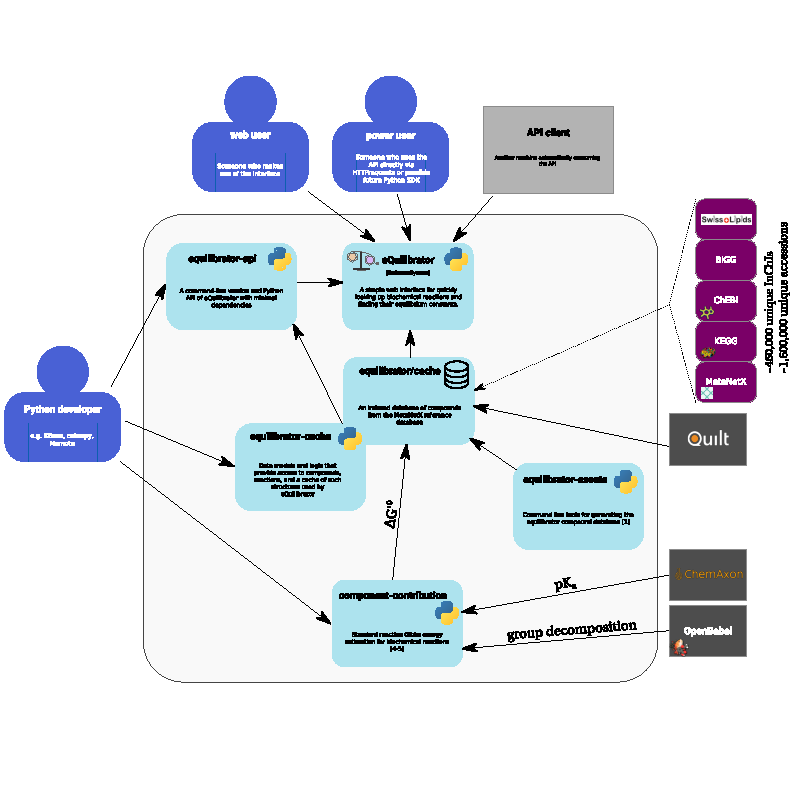
\includegraphics[width=\textwidth]{equilibrator_3_0.pdf}
    \caption{The design of the eQuilibrator 3.0 suite}
    \label{fig:eq3_design}
\end{figure}

\subsubsection{Support for multiple compound databases}
MetaNetX, KEGG, ChEBI, BiGG, Swiss Lipids (see Figure \ref{fig:eq3_design}).

\subsubsection{Automatic annotation of COBRA models with $\Delta G'^\circ$ values}
\textbf{Needs to be implemented first.}

\subsection{Fast Calculation of Gibbs energies using Component Contributions}

It is a specific challenge to use the Component Contribution (CC) method in a website such as eQuilibrator, since uncertainty calculations must be made on-the-fly, but the math for CC was developed as a one-step calculation for thousands of reactions in a model. The time it takes to run CC even for a single reaction is too long to be useful for a website.

Therefore, we need to come up with a pre-processing scheme which will probably involve several intermediate matrices in-memory and the remaining calculations will be minimal.

\subsubsection{Standard Component Contribution}
The standard CC method, is summarized by this formula for $\Delta_{r}G_{cc,X}^{\circ}$ -- the vector of estimated standard Gibbs energies:
\begin{eqnarray}\label{eq:cc}
\Delta_{r}G_{cc,X}^{\circ} = X^{\top} 
\left[ 
	\PRmat{S} \left(S^{\top}\right)^{+} +
	\PNmat{S^\top} \Gmat \left(S^{\top}\Gmat\right)^{+}
\right]
\cdot\Delta_{r}G_{obs}^{\circ}
\end{eqnarray}
where $X$ is the stoichiometric matrix of the set of reactions we wish to estimate, $S$ is the stoichiometric matrix of the training data-set, $\Gmat$ is the group incidence matrix, and $\Delta_{r}G_{obs}^{\circ}$ are the observed chemical Gibbs energies of the training set reactions. The orthogonal projections $P_{\mathcal{R}\left(S\right)}$ and $P_{\mathcal{N}(S^{\top})}$ are the projections on the range of $S$ and the null-space of $S^\top$ respectively. The $()^{+}$ sign represents the matrix pseudo-inverse.

The full co-variance matrix of the uncertainty in $\Delta_{r}G_{cc,X}^{\circ}$ is given by:
\begin{eqnarray}
\Sigma_{cc,X} &=& X^{\top} \left[ \alpha_{rc}\cdot C_{rc} + \alpha_{gc}\cdot C_{gc} + \infty\cdot C_{\infty}  \right] X \label{eq:full_u}
\end{eqnarray}
where
\begin{eqnarray}
\alpha_{rc} &\equiv& \frac{||e_{rc}||^{2}}{n-\mbox{rank}(S)} \\
\alpha_{gc} &\equiv& \frac{||e_{gc}||^{2}}{n-\mbox{rank}(S^{\top}\Gmat)} \\
C_{rc} & \equiv & \PRmat{S} \left(SS^{\top}\right)^{+} \PRmat{S} \label{eq:c_rc}\\
C_{gc} & \equiv & \PNmat{S^\top} \Gmat \left(\Gmat^{\top}SS^{\top}\Gmat\right)^{+} \Gmat^{\top} \PNmat{S^\top} \\
C_{\infty} & \equiv & \Gmat \PNmat{S^\top\Gmat} \Gmat^{\top}
\end{eqnarray}
and $e_{rc}$ and $e_{gc}$ are the residuals of the reactant and group contribution regressions.

Note that the diagonal values in $\Sigma_{cc,X}$ are the squared standard errors of the estimates of single reactions.


\subsubsection{Calculating Gibbs energy estimates on-the-fly}

What happens when we want to estimate the Gibbs energy of reactions with reactants that are not in $S$? The long way would be to augment $S$, $\Gmat$ and $X$ with more rows that would correspond to the new compounds. Note that if we do not have a group decomposition of one of these new compounds, there is no way to make the estimation (we cannot add ``group columns'' like we did for compounds in the training set). Fortunately, we will soon see that the effect of the added rows on the calculation is minimal, and it is easy to do the pre-processing trick we need.

Let $\Gmat'$ be the group incidence matrix of only the new compounds, and $X'$ the stoichiometric coefficients of the new compounds. Then the new matrices we need to use for CC are:

\begin{eqnarray}
	\bar{X} & \equiv & \left( \begin{array}{c} X \\ \hline X' \end{array} \right) \\
	\bar{S} & \equiv & \left( \begin{array}{c} S \\ \hline 0 \end{array} \right) \\
	\bar{\Gmat} & \equiv & \left( \begin{array}{c} \Gmat \\ \hline \Gmat'\end{array} \right)
\end{eqnarray}
It is easy to see that $\bar{S}^\top \bar{\Gmat} = S^\top \Gmat$. Since we added only zeros to $S$, the range will not change, and the null-space of $S^\top$ will include all the new rows. Therefore
\begin{eqnarray}
	\PRmat{\bar{S}} & \equiv & \left( \begin{array}{c|c} \PRmat{S} & 0 \\ \hline 0 & 0 \end{array} \right)	 \\
	\PNmat{\bar{S}^\top} & \equiv & \left( \begin{array}{c|c} \PNmat{S^\top} & 0 \\ \hline 0 & I \end{array} \right)
\end{eqnarray}

So, the left term in the parentheses of equation \ref{eq:cc} (i.e., the one we call reactant contribution) will not change at all. The right term (group contribution) can be rewritten in block-matrix form:
\begin{eqnarray}\label{eq:P_N_ST_G}
\PNmat{\bar{S}^\top} \bar{\Gmat} &=& 
\left( \begin{array}{c|c} \PNmat{S^\top} & 0 \\ \hline 0 & I \end{array} \right)
\left( \begin{array}{c} \Gmat \\ \hline \Gmat'\end{array} \right)
 = \left( \begin{array}{c} \PNmat{S^\top} \Gmat \\ \hline \Gmat' \end{array} \right)
\end{eqnarray}

Plugging it back into equation \ref{eq:cc} we get:
\begin{eqnarray}
\Delta_{r}G_{cc,\bar{X}}^{\circ} &=& 
    X^\top \left[
	\PRmat{S} \left(S^{\top}\right)^{+} +
	\PNmat{S^\top} \Gmat  \left(S^{\top}\Gmat\right)^{+} \right]\Delta_{r}G_{obs}^{\circ} ~+~ \nonumber\\ && 
	X'^\top \Gmat' \left(S^{\top}\Gmat\right)^{+} \Delta_{r}G_{obs}^{\circ}
\end{eqnarray}
We can define the pre-processing vectors (which depend only on the training data and not on the reaction we wish to estimate) as:
\begin{eqnarray}
	v_{r} &\equiv&
	\left[
		\PRmat{S} \left(S^{\top}\right)^{+} + 
		\PNmat{S^\top} \Gmat \left(S^{\top}\Gmat\right)^{+}
	\right]
	\Delta_{r}G_{obs}^{\circ}
\\
	v_g &\equiv& \left(S^{\top}\Gmat\right)^{+} \Delta_{r}G_{obs}^{\circ}
\end{eqnarray}
and get that
\begin{eqnarray}
\Delta_{r}G_{cc,\bar{X}}^{\circ} &=& X^\top v_r ~+~ X'^\top \Gmat' v_g
\end{eqnarray}

\subsubsection{Calculating uncertainty estimates on-the-fly}
If we look again at equation \ref{eq:c_rc}, it's obvious that $\bar{C}_{rc} = C_{rc}$ is not affected by the new compounds in $x'$, besides some zero-padding for adjusting its size. From what we saw in the previous section, $\bar{S}^\top \bar{\Gmat} = S^\top \Gmat$ and using \ref{eq:P_N_ST_G} we can conclude that:
\begin{eqnarray}
	\bar{C}_{gc} &=& \left( \begin{array}{c} \PNmat{S^\top} \Gmat \\ \hline \Gmat' \end{array} \right)
	\left(\Gmat^{\top}SS^{\top}\Gmat\right)^{+} 
	\left( \begin{array}{c|c} \Gmat^\top \PNmat{S^\top} & \Gmat'^\top \end{array} \right) 
\\
&=&
\left( \begin{array}{c|c} C_{gc} & \PNmat{S^\top} \Gmat \left(\Gmat^{\top}SS^{\top}\Gmat\right)^{+} \Gmat'^\top \\ \hline \Gmat' \left(\Gmat^{\top}SS^{\top}\Gmat\right)^{+} \Gmat^\top \PNmat{S^\top} & \Gmat'\left(\Gmat^{\top}SS^{\top}\Gmat\right)^{+} \Gmat'^\top \end{array} \right)
\end{eqnarray}
and the third term in equation \ref{eq:full_u} will change to:
\begin{eqnarray}
	\bar{C}_{\infty} &=& 
		\left(\begin{array}{c} \Gmat \\ \hline \Gmat' \end{array}\right)
		\PNmat{S^\top\Gmat}
		\left(\begin{array}{c|c} \Gmat^\top & \Gmat'^\top \end{array}\right)
\\ &=&
	\left(\begin{array}{c|c}
		C_\infty &
		\Gmat \PNmat{S^\top\Gmat} \Gmat'^\top \\ \hline
		\Gmat' \PNmat{S^\top\Gmat} \Gmat^\top &
		\Gmat' \PNmat{S^\top\Gmat} \Gmat'^\top
 \end{array}\right)
\end{eqnarray}

Finally, we define $\Gamma \equiv \left(\Gmat^{\top}SS^{\top}\Gmat\right)^{+}$ and then we can derive the following explicit formula for the uncertainty in $\Delta_{r}G_{cc,\bar{X}}^{\circ}$:
\begin{eqnarray}
\Sigma_{cc,\bar{X}}
&=& 
\bar{X}^{\top} \left[ \alpha_{rc}\cdot \bar{C}_{rc} + \alpha_{gc}\cdot \bar{C}_{gc} + \infty\cdot \bar{C}_{\infty}  \right] \bar{X}
\\ &=&
\alpha_{rc} \cdot X^{\top} C_{rc} X + \alpha_{gc} \cdot \bar{X}^{\top} \bar{C}_{gc} \bar{X} + \infty \cdot \bar{X}^{\top} \bar{C}_{\infty} \bar{X}
\nonumber\\ &=&
\alpha_{rc} \cdot X^{\top} C_{rc} X ~~+
\nonumber\\ &&
\alpha_{gc} \cdot \left( \begin{array}{c|c} X^\top & X'^\top \end{array} \right)
\left( \begin{array}{c|c}
		C_{gc} &
		\PNmat{S^\top} \Gmat ~ \Gamma ~ \Gmat'^\top \\ \hline
		\Gmat' ~ \Gamma ~ \Gmat^\top \PNmat{S^\top} &
		\Gmat' ~ \Gamma ~ \Gmat'^\top
	\end{array} \right)
 \left( \begin{array}{c} X \\ \hline X' \end{array} \right)
\nonumber\\ &&+~
\infty \cdot \left( \begin{array}{c|c} X^\top & X'^\top \end{array} \right)
\left( \begin{array}{c|c}
		C_\infty &
		\Gmat \PNmat{S^\top\Gmat} \Gmat'^\top \\ \hline
		\Gmat' \PNmat{S^\top\Gmat} \Gmat^\top &
		\Gmat' \PNmat{S^\top\Gmat} \Gmat'^\top
 \end{array}\right) \left( \begin{array}{c} X \\ \hline X' \end{array} \right)
\nonumber\\ &=&
\alpha_{rc} \cdot X^{\top} C_{rc} X ~~+
\nonumber\\ &&
\alpha_{gc} \cdot \left(
	X^\top C_{gc} X +
	X^\top \PNmat{S^\top} \Gmat  \Gamma \Gmat'^\top                X' + 
	X'^\top               \Gmat' \Gamma \Gmat^\top  \PNmat{S^\top} X  +
	X'^\top               \Gmat' \Gamma \Gmat'^\top                X'
\right)
\nonumber\\ &&+~
\infty \cdot \left(
	X^\top C_{\infty} X +
	X^\top \Gmat \PNmat{S^\top\Gmat} \Gmat'^\top X' +
	X'^\top \Gmat' \PNmat{S^\top\Gmat} \Gmat^\top X +
	X'^\top \Gmat' \PNmat{S^\top\Gmat} \Gmat'^\top X'
\right)
\nonumber
\label{eq:standard_error}
\end{eqnarray}

So, as a pre-processing step, we can calculate the following matrices:
\begin{eqnarray}
	C_1 &=& \alpha_{rc} \cdot C_{rc} + \alpha_{gc} \cdot C_{gc} + \infty \cdot C_\infty \\
	C_2 &=& \alpha_{gc} \cdot \PNmat{S^\top} \Gmat \Gamma + \infty \cdot \Gmat \PNmat{S^\top\Gmat} \\
	C_3 &=& \alpha_{gc} \cdot \Gamma + \infty \cdot \PNmat{S^\top\Gmat} 
\end{eqnarray}
And therefore the on-the-fly calculation of the standard error will be:
\begin{eqnarray}
	\Sigma_{cc,\bar{X}} &=& X^\top C_1 X + X^\top C_2 G + G^\top C_2^\top X + G^\top C_3 G
\end{eqnarray}
where $G \equiv \Gmat'^\top X'$. Note that the sizes of the $C$ matrices are:
\begin{eqnarray}
	C_1 \in \mathbb{R}^{N_c \times N_c} \\
	C_2 \in \mathbb{R}^{N_c \times N_g} \\
	C_3 \in \mathbb{R}^{N_g \times N_g}
\end{eqnarray}
Assuming $N_c = 600$ and $N_g = 200$, we'll need to store 520,000 floats which is only about 2MB.

\subsection{Sampling from a multivariate Gaussian}
Consider a $D$-dimensional random variable that is Normally distributed with mean $\mu$ and co-variance $\Sigma$.

If we have a 1-dimensional random Gaussian sampler, we can sample from the multivariate distribution by sampling $D$ times and then stretching and rotating the vector according to $\Sigma$. Specifically, we define the square root of the co-variance matrix as
\begin{eqnarray}
	\sqrt{\Sigma} = U \cdot \sqrt{S} \cdot U^\top
\end{eqnarray}
where where $S$ is a diagonal real matrix and $U$ is unitary which are given by the Singular Value Decomposition (SVD) of the co-variance matrix, i.e. $\Sigma = U \cdot S \cdot U^\top$ (note that $\Sigma$ is Hermitian and thus diagonalizable with real eigenvalues).

If $\forall i :~ y_i \sim \mathcal{N}(0, 1)$ and we define $z \equiv \mu + y \cdot \sqrt{\Sigma}$ then
\begin{eqnarray}
z \sim \mathcal{N}(\mu, \Sigma)
\end{eqnarray}

The same approach can be applied for setting hard linear constraints on a the original variable in the context of linear programming. We define the auxiliary variable $y \in [-1, 1]^D$ replace the random variable by the expression $\mu + K \cdot y \cdot \sqrt{\Sigma}$, where $K$ is a parameter of how loose we want the constraints to be (typically, we use the value $3$).

This approach is easily applied to linear problems that utilize thermodynamic constraints, and use the standard Gibbs energies provided by Component Contribution. The vector of $\Delta_{r}G^{\circ}$ for a given problem should be constrained to:
$\Delta_{r}G^{\circ} = \Delta_{r}G_{cc,\bar{X}}^{\circ} + 3 \cdot y \cdot \sqrt{\Sigma}_{cc,\bar{X}}$
\end{document}
